% !TEX root = mainthesis.tex

%Chapter 3


\renewcommand{\thechapter}{3}

\chapter{Manipulation and detection of ultra-cold atoms}
\label{ch:Ch3}

All of the experiments described in this thesis were performed using ultracold clouds of $\Rb87$. Both the cooling and trapping of atoms as well as the engineering of interesting potentials and detection of atoms rely on the interaction of atoms with electromagnetic fields as well as with static and oscillating magnetic fields. 

In this Chapter I describe the techniques and interactions that make our experiments possible. This Chapter is not meant to be an extensive survey of atomic physics but rather covers the topics that are most relevant to the experiments presented in this thesis. The references I included are helpful if the reader is interested in the details of the derivations or wants to expand on a given topic. I start by describing the electronic structure of $\Rb87$. Then I review the interactions of atoms with magnetic fields which allows us to shift the energies of different atomic states. I describe the foundations of atom-light interactions that make possible both laser cooling and trapping of atoms and gives rise to Raman induced transitions. Finally I discuss the absorption imaging technique that we use to detect atoms after all our experiments are performed. 

\section{Electronic structure of $^{87}$Rb}
\label{sec:electronic_structure}

Rb is an Alkali metal (also Li, which exists in our vacuum chamber but was never used). Alkali metals correspond to the first group (leftmost column) of the periodic table and are characterized by having a single valence electron, which makes the description of their internal structure much simpler than that of other elements. We can describe the state of an electron in an atom by its angular momentum $\mathbf{\hat{L}}$ and its spin $\mathbf{\hat S}$. Because of Pauli's exclusion principle there can not be two electrons with the same quantum numbers and in multi-electron atoms they tend to fill `shells' of different angular momentum values, historically labeled by the letters $S,\ P,\ D,\ F,\ ...$\footnote{This terms were used to describe the lines in the emission spectra when they were first discovered. $S$ stands for sharp, $P$ for principal $D$ for diffuse and $F$ for further noted} (corresponding to $L=1,\ 2,\ 3,\ 4,\ ...$). In particular Rb has 4 filled shells and one electron in the $5S$ 
shell, where the number $5$ corresponds to the principal quantum number $n$. Figure \note{TODO: make figure of atomic energy levels} shows the energy levels of the ground state $5S$ and its closest $5P$ orbital. %In the absence of interactions, the $m_l$ sublevels within an orbital are degenerate.

The atomic level structure is modified by relativistic effects. In particular the relativistic treatment of the electron's motion gives rise to an interaction between the electron's intrinsic magnetic moment (the spin) $\mathbf{\hat S}$ and the orbital angular momentum $\mathbf{\hat L}$. This spin-orbit coupling interaction $\hat H_{\rm {fs}} \propto \mathbf{L}\cdot\mathbf{S}$ causes the fine structure splitting of the electronic orbitals into levels with different total electronic angular momentum $\mathbf{J}=\mathbf{\hat L}\cdot\mathbf{\hat S}$. Figure~\ref{fig:fs_hfs}b show the $5^2S_{1/2}$, $5^2P_{1/2}$ and $5^2P{3/2}$ electronic configurations that arise from this splitting, where the subscript indicates the value of $J$. For $S$ ($L=0$) orbitals $J=1/2$ is the only possible value and the levels are not split. For the $P$ orbital ($L=1$) $J$ and a single electron with $S=1/2$, $J$ can be $1/2$ or $3/2$ and the $P$ orbital splits into two levels. The $5S_{1/2}\rightarrow 5P_{1/2}$ is known as the D1 line and has wavelength $\lambda=\unit[794.979]{nm}$ and $5S_{1/2}\rightarrow 5P_{3/2}$ transition is known as the D2 line and has $\lambda=\unit[790.241]{nm}$ \cite{Steck}. 

The atomic level structure gets further modified by the magnetic interaction of the electronic magnetic flux density with the nuclear spin $\mathbf{I}$. This is another kind of spin-orbit interaction that gives rise to the hyperfine splitting of the atomic levels which can be described by the Hamiltonian $\hat H_{\rm{hfs}} = A_{\rm{hfs}}\mathbf{I}\cdot\mathbf{J}$. A complete derivation of $\hat H_{\rm{hfs}}$ can be found in~\cite{schwartz_theory_1955}. The hyperfine levels correspond to different values of the total angular momentum $\hat F=\hat J+\hat I$. For $\Rb87$ $I=3/2$~\cite{Steck} which results in the level structure shown in Figure~\ref{fig:fs_hfs}c 

\note{TODO: talk about cooling and repumping transitions which is relevant for the absorption imaging section.}

\section{Interaction between atoms and magnetic fields}
\label{sec:zeeman_effect}

Atoms have have an intrinsic magnetic moment that is given by the sum of nuclear and electronic moments
%
\begin{equation}
	\boldsymbol{\hat \mu}=-\frac{g_J\mu_B}{\hbar} \mathbf{\hat J}+\frac{g_I\mu_N}{\hbar}\mathbf{\hat I}=\frac{\mu_B g_F}{\hbar} \mathbf{\hat F}
\end{equation}
%
where $\mu_B$ is the Bohr magneton, $\mu_N$ \footnote{$\mu_N\ll\mu_B$ and therefore $\boldsymbol{\hat \mu}\approx-\mu_Bg_J/\hbar\mathbf{\hat J}$} is the nuclear magneton and $g_J$, $g_I$ and $g_F$ are the Land\'e $g$-factors corresponding to the electronic, nuclear and total angular momentum. In the presence of an external magnetic field $\mathbf B$, the internal levels of an atom get modified due to the Zeeman~\cite{Zeeman_effect} interaction
%
\begin{equation}
	\hat{H}_{\rm{Zeeman}}=-\boldsymbol{\hat \mu}\cdot\mathbf{B}
	\label{eq:zeeman_hamiltonian}
\end{equation}
%
which has the effect of lifting the degeneracy of the different $m_F$ states. We take advantage of this effect for making (state-dependent) magnetic traps for the atoms by using magnetic field gradients and for the experiments presented in Chapters~\ref{ch:Fourier_spectroscopy},~\ref{ch:clock_states} and \ref{ch:Rashba} the shifts in the $m_F$ energies allowed us to treat each state as a pseudospin that we then coherently manipulated using the techniques described in Section~\ref{sec:quantum_coherent_dynamics}.

The total energy shifts are calculated by diagonalizing the full atomic Hamiltonian including the fine and hyperfine structure terms. For a small magnetic field the Zeeman term can be treated as a perturbation and the energy split is linear with the magnitude of the field $\Delta E_{\rm{Zeeman}}=g_F\mu_B m_FB$, what is known as the `linear Zeeman regime' where $F$ and $m_F$ are good quantum numbers. In contrast, in the `Pachen-Back regime' large magnetic fields the Zeeman term dominates over the fine and hyperfine terms and therefore the good quantum numbers of the system are $J$ and $m_J$. Our experiments typically operate in an intermediate regime ($B\sim 10-30\,\rm{G}$)energies where the magnetic field and as a result the energy of $m_F=0$ gets a small shift in energy that is quadratic in $B$. For atoms in $F=1$ we define this quadratic Zeeman shift as $\epsilon=E_0-(E_{+1}-E_{-1})/2$, where $E_{m_F}$ is the Zeeman shift for state $m_F$.

For the particular case of $J=1/2$ (like the ground state of Alkalis) the Zeeman energies can be found analytically using the Breit-Rabi formula~\cite{breit_measurement_1931}
%
\begin{equation}
	E_{m_F}=-\frac{1}{2(2I+1)}+\frac{\mu_Bg_Im_FB}{\Delta E_{\rm{hf}}}+\frac{1}{2}\sqrt{1+\frac{4m_F}{2I+1}x+x^2},
	\label{eq:Breit_rabi}
\end{equation}
%
where $\Delta E_{\rm{hf}}=A_{\rm{hf}}(J+1/2)$ and $x=(g_J-g_I)\mu_B B_z/\Delta E_{\rm{hf}}$. Figure \note{TODO:make figure} shows the energies of the $m_F$ levels for the $F=1$ and $F=2$ manifolds of $\Rb87$.

\section{Interaction between atoms and electric fields}
\label{sec:atom-lignt_interactio n}

In this section I will discuss the interaction between atoms and electromagnetic radiation (light). After laying the foundations I will discuss applications using off-resonant light such as optical dipole traps and Raman transitions. I will not cover laser cooling which has been covered extensively in the literature~\cite{metcalf_deceleration_1999,phillips_nobel_1998} and PhD theses from previous lab members~\cite{CampbellThesis,PriceThesis}. 

In the presence of an electric field $\mathbf E$ an atom can become polarized and therefore its energy levels get modified by the Stark effect~\cite{stark_beobachtungen_1914}. If the electric field is spatially uniform with respect to the atom's size we consider the electric field as a classical object and its effect on the atom can be described by the the Hamiltonian~\cite{Cohen-Tanoudji}  
%
\begin{equation}
\hat{H}_{\rm{dip}} = -\mathbf{\hat d}\cdot\mathbf{E},
\label{eq:dipole_ham}	
\end{equation}
%
where $\mathbf{\hat d}=-e\sum_j r_j$ is the atomic dipole operator, $e$ is the electron charge and $\hat r_j$ are the position operators of the atom's electrons relative to the center of mas of the atom. This approximation, known as the dipole approximation, is valid for electromagnetic radiation when the wavelength is much larger than the size of an atom $\lambda\gg r_{\rm{atom}}$~\cite{SteckTextbook}. 

For a coherent electromagnetic field $\mathbf{E}(\omega,t)$ with angular frequency $\omega$, the dipole Hamiltonian can be written in terms of a dynamic polarizability
%
\begin{equation}
	\hat{H}_{\rm{dip}}=-\alpha_{\mu\nu}(\omega)E_{\mu}^{(+)}E_{\nu}^{(-)}
\end{equation}
%
where $\mathbf{E}^{(\pm)}$ are the possitive/negative frequency components of the field. $\alpha_{\mu\nu}(\omega)$ can be found by looking at the (time averaged) shift in the energy of the a given state state using second order time-dependent perturbation theory~\cite{SteckTextbook,deutsch_quantum_2010}. For the ground state $\ket{g}$ the polarizability takes the form
%
\begin{equation}
	\alpha_{\mu\nu}(\omega)=\sum_j\frac{2\omega_{jg}\bra{g}d_\mu\ket{e_j}\bra{e_j}d_\nu\ket{e_j}}{\hbar(\omega_{jg}^2-\omega^2)},
\end{equation}
%
where $\ket{e_j}$ represent the excited states and $\omega_{jg}=(E_j-E_g)/\hbar$. The dipole operator is a rank-1 tensor and can be represented by 3 irreducible tensor operators\footnote{A rank $k$ tensor can be represented by $2k+1$ irreducible tensor operators, which are collection of operators that transforms under
rotations like the spherical harmonics $Y_{kq}(\theta, \phi)$} (see~\cite{SteckTextbook} for a complete derivation). In the limit of small magnetic fields so that $F$ and $m_F$ are good quantum numbers describing the state of the atom $\ket{n, F, m_F}$ the dipole Hamiltonian in this representation takes a convenient form
%
\begin{align}
	\hat{H}_{\rm{dip}}= &\alpha^{(0)}(\omega)(\mathbf{E}^{(-)}\cdot\mathbf{E}^{(+)}) 
	+\alpha^{(1)}(\mathbf{E}^{(-)}\times\mathbf{E}^{(+)})\cdot\mathbf{\hat{F}}  \nonumber \\ 
	&+ \alpha^{(2)}E_i^{(-)}E_j^{(+)}	\left(\frac{1}{2}(F_iF_j+F_jF_i)-\frac{1}{3}\mathbf{\hat F}^2\delta_{i,j}\right)\Big],
	\label{eq:light_matter_coupling}
\end{align}
%
where $\alpha^{(0)}$, $\alpha^{(1)}$ and $\alpha^{(2)}$ are the scalar, vector and tensor polarizabilities respectively and $\hat{\mathbf{F}}$ is the total angular momentum operator. For all our experiments $\alpha^{(2)}$ is very small so I will limit the discussion to the effect of the first two terms. The scalar term is responsible for the dipole force that allow us to trap atoms using off-resonant light and the vector component is necessary for engineering spin-orbit coupling through Raman transitions and other spin-dependent potentials. 

\subsection{Scalar polarizability}
\label{sec:scalar_light_shift}

The scalar polarizability takes the form
%
\begin{equation}
	\alpha^{(0)}=\sum_j\frac{2\omega_{jg}\bra{g}\mathbf{d}\cdot\hat{\epsilon}\ket{e_j}\vert^2}{\hbar(\omega_{jg}^2-\omega^2)},
\end{equation}
%
where $\hat{\epsilon}$ represents the polarization vector of the light. The matrix element can be expressed in terms of the Clebsch-Gordan coefficients and the reduced matrix element using the Wigner-Eckart theorem~\cite{Sakurai}. For the ground state of an Alkali atom ($J=1/2$) the expression above gets simplified to
%
\begin{equation}
	\alpha^{(0)}\approx\sum_{J'}\frac{2\omega_{JJ'}\vert\langle J=1/2 \| \mathbf{d}\|J'\rangle\vert^2}{3\hbar(\omega_{JJ'}^2-\omega^2)}.
\end{equation}

The dipole matrix elements needed to compute the polarizability are related to the transition scattering rate via Fermi's golden rule~\cite{Sakurai,SteckTextbook}
\begin{equation}
	\Gamma_{JJ'}=\frac{\omega_{JJ'}^2}{3\pi\epsilon_0\hbar c^3}\frac{2J+1}{2J'+1}\vert\langle J \| \mathbf{d}\|J'\rangle\vert^2,
\end{equation}
%
and combining this with the expression for the intensity of the electric field $I(\r)=2\epsilon_0c\vert \mathbf{E}(\r)\vert^2$ it can be shown that for linearly polarized light the energy of the ground state manifold is shifted by
\begin{equation}
	U(\omega,\r)=-\frac{\pi c^2 I(\r)}{2}\left[ \frac{\Gamma_{\rm{D1}}}{\omega_{\rm{D1}}^2}\left(\frac{1}{\omega+\omega_{\rm{D1}}}-\frac{1}{\omega-\omega_{\rm{D1}}}\right)+\frac{2\Gamma_{\rm{D2}}}{\omega_{\rm{D2}}^2}\left(\frac{1}{\omega+\omega_{\rm{D2}}}-\frac{1}{\omega-\omega_{\rm{D2}}}\right)\right],
\end{equation}
%
where only the the most significant contribution from the closest transitions  (the D1 and D2 lines) are included. Here $U(\r)$ is related to the real part of the polarizability which is in fact a complex valued number. So far I have only considered the real part by assuming the excited states have an infinitely long lifetime. However, in reality the atom can spontaneously emit photons and decay. This exponential decay can be accounted for by adding an imaginary contribution to the energies $\omega_D\rightarrow\omega_D+i\Gamma_D\omega^3/\omega_D^3$ of the D1 and D2 transitions~\cite{grimm_optical_2000}. The scattering rate is related to the imaginary part of the polarizability and is given by
%
\begin{equation}
	\Gamma(\omega,\r)=\frac{\pi c^2I(\r)}{2\hbar}\left[ \frac{\Gamma_{\rm{D1}}\omega^3}{\omega_{\rm{D1}}^6}\left(\frac{1}{\omega+\omega_{\rm{D1}}}-\frac{1}{\omega-\omega_{\rm{D1}}}\right)^2+\frac{2\Gamma_{\rm{D2}}\omega^3}{\omega_{\rm{D2}}^6}\left(\frac{1}{\omega+\omega_{\rm{D2}}}-\frac{1}{\omega-\omega_{\rm{D2}}}\right)^2\right]
	\label{eq:scattering}
\end{equation}

The energy shift $U(\omega,\r)$ is a conservative term and is related to dipole trapping while the scattering term $\Gamma(\omega,\r)$ is dissipative and is important for laser cooling. In the context of engineering potentials for ultracold atoms with off-resonant light, the scattering is translated into heating because every time an atom emits a photon with angular frequency $\omega_L$ it gets a recoil momentum $\hbar\k_L$.  

If the frequency $\omega$ satisfies the relation $\omega+\omega_{\rm D}\gg\omega-\omega_{\rm D}$ we can neglect the terms proportional to $1/(\omega+\omega_{\rm D})$, an approximation typically known as the rotating wave approximation (RWA). If the RWA is valid then the frequency dependence of both the energy shifts and the scattering rates will be given by the detuning from the D1 and D2 transitions. 

\subsubsection{Optical trapping}
One important application of the scalar light-shift is to create optical traps for our clouds of ultracold atoms. The use optical fields with non-uniform spatial intensity can generate traps (and anti-traps) for the atoms which experience a force proportional to the intensity gradient $F_{\rm{dip}}=-\nabla U(\r)$.  \note{TODO: make nice figure of dipole trap?}. The production of BECs in our lab relies on the use of focused Gaussian laser beams with $\lambda=\unit[1064]{nm}$.  The intensity profile of a focused Gaussian beam propagating along $\ez$ is given by 
%
\begin{equation}
 	I(x,y,z) = \frac{2P}{\pi\omega^2(z)}e^{-\frac{x^2+y^2}{\omega^2(z)}}
 \end{equation} 
 %
 where $P$ is the total power of the beam and the $1/e^2$ radius is given by $w(z)=w_0\sqrt{1+z^2/z_R^2}$ where the minimum radius $w_0$ is known as the waist and $z_R=\pi\omega_0^2/\lambda$ is the Rayleleigh range. If the extent of an atomic cloud is small compared to the size of the beam we can perform a Taylor expansion around $\r=0$ to obtain the trapping potential
 %
 \begin{equation}
 	U(\r) = -U_0\left(1-2\frac{x^2+y^2}{\omega_0^2}-\frac{z^2}{z_R^2}\right).
 \end{equation}
%
The oscillation frequencies of the trap along the radial direction are $\omega_r=(4U_0/m\omega_0^2)^{1/2}$ and along the axial direction $\omega_z=(2U_0/mz_R)^{1/2}$. The beam waist is usually much smaller than the Rayleigh range ($\omega_0\sim \unit[50-150]{nm}$ for my experiments) and therefore the trap is much stronger along the axial direction. To get around this we use a `crossed dipole trap' which is formed by a combination of two cross-polarized\footnote{The beams are cross-polarized to avoid interference between them} focused Gaussian beams propagating along perpendicular axes, ensuring that we get good confinement of atoms along all spatial directions. 

For a given trapping potential $U(\r)$, the density distribution of a thermal ensamble is
\begin{equation}
	n(\r) = n_0 e^{-\frac{U(\r)}{k_BT}}.
\end{equation}
%
The temperature $T$ can be derived from the density distribution. For a 3D harmonic trap
%
\begin{equation}
	n(\r)=n_0e^{-(\frac{x^2}{2\sigma_x^2}+\frac{y^2}{2\sigma_y^2}+\frac{z^2}{2\sigma_z^2})},
\end{equation}
%
where $\sigma_i=\omega_i^{-1}\sqrt{k_BT/m}$. Using the equipartition theorem we find that the spatial extension of the cloud and the temperature are related by 
%
\begin{equation}
	T=\frac{m}{k_B}\sigma_i^2\omega_i^2
\end{equation}

\note{TODO: figure of dipole traps}

\note{TODO: talk about magic wavelength}

\subsection{Effective magnetic fields from vector polarizability}
\label{sec:}

Recall the Zeeman Hamiltonian introduced in Section~\ref{sec:zeeman_effect}. The term proportional to the vector polarizability in Equation~\ref{eq:light_matter_coupling} looks very similar to Equation~\ref{eq:zeeman_hamiltonian} for an effective magnetic field
%
\begin{equation}
	\mathbf{B}_{\rm{eff}}=-\frac{i\hbar}{\mu_Bg_J}\alpha^{(1)}(\mathbf{E}^*\times\mathbf{E}).
\end{equation}

For Alkali atoms the vector poarizability takes the form
%
\begin{equation}
	\alpha^{(1)}= \frac{2\alpha^{(0)}\Delta_{\rm{fs}}}{3(\tilde{E}-\hbar\omega)}
\end{equation}
%
where $\Delta_{\rm{fs}}=3A_{\rm{fs}}/2$ and $\tilde{E}=(2E_{\rm{D_1}}+E_{\rm{D2}})$. For the magnetic field magnitudes and light intensities that we typically operate at the vector light shift is small compared to the Zeeman splitting and therefore it can be treated as a perturbation to the hyperfine Hamiltonian
%
\begin{equation}
 	\hat{H}_{\rm{eff}}=\frac{\mu_Bg_F}{\hbar}\mathbf{B}_{\rm{eff}}\cdot\mathbf{\hat F}
 \end{equation} 

\subsection{Raman coupling}

The vector light shift enables the realization of various spin dependent potentials in the lab. In the experiments presented in Chapters~\ref{ch:Fourier_spectroscopy} and \ref{ch:Rashba} I used combinations of cross polarized laser beams such that for the total electric field $\mathbf{E}^*\times\mathbf{E}\neq0$ to induce Raman tranisitions. A Raman transition is a two-photon process between two ground states that uses an intermediate state that is off-resonantly coupled as is shown in Figure~\ref{fig:Raman_coupling}a. Because the intermediate state is far detuned it can be adiabatically eliminated~\cite{han_raman_2013} so the system is effectively treated as a two level system. In our experiments we typically couple the $m_F$ levels of the $F=1$ manifold after applying a bias magnetic field such that $\epsilon$ is non-negligible. I describe the most simple case which considers coupling only two levels, in the later Chapters of the thesis this scheme is extended to couple multiple levels. 

\begin{figure*}[htb]
\begin{center}
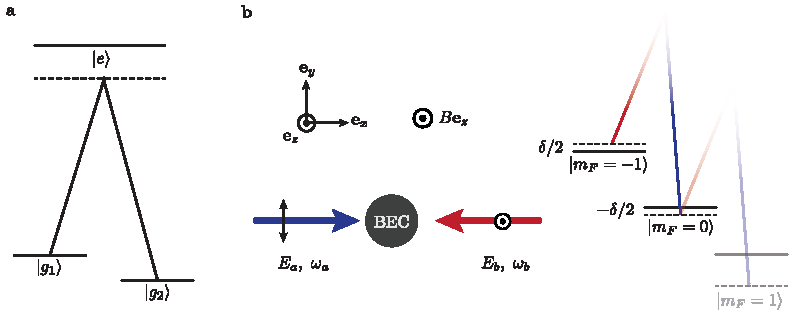
\includegraphics[]{Figures/Chapter3/Raman_coupling.pdf}
\caption[Raman coupling with two-photon transitions]{\note{TODO:write caption}}
\label{fig:Raman_coupling}
\end{center}
\end{figure*}

Consider two laser beams counter propagating along $\ex$ and with polarizations along $\ey$ and $\ez$ as is shown in Figure~\ref{fig:Raman_coupling}b. The electric field from the Raman beams is given by
%
\begin{equation}
  \mathbf{E}(x,t) = E_a\cos(k_a x-\omega_at)\e_y + E_b\cos(k_b x+\omega_bt)\ez,
\end{equation} 
%
and consequently 
%
\begin{equation}
	\mathbf{E}^*\times\mathbf{E} = 2i E_a E_b\cos(2\kl x-\Delta\omega t)\ex,
\end{equation}
%
where $\Delta\omega=\omega_a-\omega_b$. The geometry and wavelength of the Raman fields determine the natural units of the system: the single photon recoil momentum $k_{\mathrm{L}}=2\pi/\lambda_{\mathrm{R}}$ and its associated recoil energy $E_{\mathrm{L}}=\hbar^2k_{\mathrm{L}}^2/2m$, as well as the direction of the recoil momentum $\mathbf{k}_{\mathrm{L}}=k_{\mathrm{L}}\ex$. For most experiments we tune $\lambda_{\mathrm{R}}=790.032\,\nm$, so that the scalar light shift is zero and the scattering rate is minimized. The Raman Hamiltonian is given by
%
\begin{equation}
	\hat{H}_{R}=\Omega\cos(2\kl x-\Delta\omega t)\fx
\end{equation}
%
where $\Omega=\alpha^{(1)}g_F E_a E_b/g_J\propto \sqrt{I_a I_b}$ is the Raman coupling strength. In a frame rotating with angular frequency $\Delta\omega$ corresponding to applying the unitary transformation $\hat{U}(t)=\exp(-i\Delta\omega t\fz)$ and neglecting the fast terms rotating at frequency $2\Delta\omega$ (applying a RWA) the transformed Hamiltonian is
%
\begin{equation}
	\hat{U}^{\dagger}\hat{H}_R\hat{U} - i\hbar\hat{U}^{\dagger}\partial_t\hat{U}=\Delta\omega \fz+\frac{\Omega}{2}\cos(2\kl x)\fx-\frac{\Omega}{2}\sin(2\kl x)\fy,
	\label{eq:basic_Raman}
\end{equation}
%
which describes a helically precessing magnetic field with period $\lambda_{\rm R}/2$ which is illustrated in Figure~\ref{fig:B_eff}.

\begin{figure*}[htb]
\begin{center}
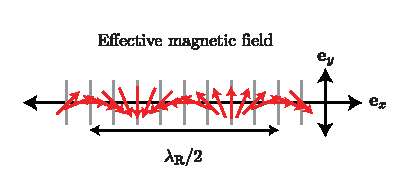
\includegraphics[]{Figures/Chapter3/B_eff.pdf}
\caption[Effective magnetic field from two cross polarized Raman laser beams]{\note{TODO: write caption}}
\label{fig:B_eff}
\end{center}
\end{figure*}

\note{TODO: the two-level stuff maybe doesn't really make much sense anymore}

\begin{figure*}[htb]
\begin{center}
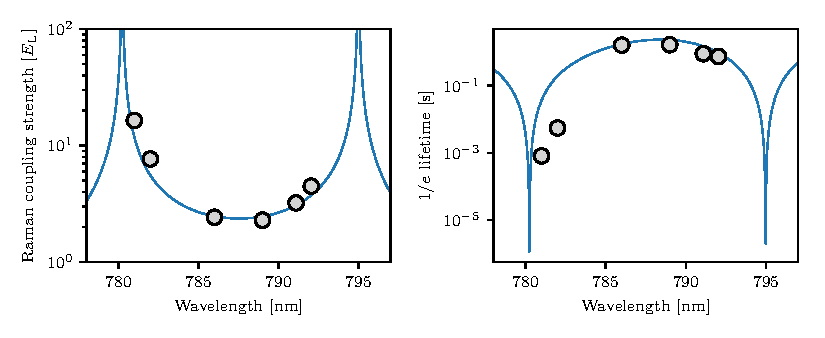
\includegraphics[]{Figures/Chapter3/Raman_vs_lambda.pdf}
\caption[Raman coupling with two-photon transitions]{\note{TODO:write caption}}
\label{fig:Raman_vs_lambda}
\end{center}
\end{figure*}

\subsection{Spin-orbit coupling}

The Raman Hamiltonian from Equation~\ref{eq:basic_Raman} can be massaged a bit more to make it look like a spin-orbit coupled\footnote{Not to be confused with the spin-orbit coupling giving rise to the fine and hyperfine structure mentioned earlier, perhaps a better name could be spin-momentum coupling} Hamiltonian that is familiar to condensed matter physicists. If we apply a spin-dependent momentum boost which is described by the unitary operator $\hat{U}(\kl)=\exp(i2\kl x \fz)$ the full Hamiltonian including the Raman coupling and the free 
%
\begin{equation}
 	\hat{H}_{\rm{SOC}} = \frac{\hbar^2}{2m}\left(\hat q_x-2\kl\fz\right)^2+\frac{\Omega}{2}\fx + \delta\fz + \hbar\epsilon\left(\mathds{1}-\frac{\fz^2}{\hbar^2}\right),
 \end{equation} 
%
where $\delta=E_-1-\Delta\omega$. We can go from an $F=1$ 3 system to an effective spin-$1/2$ system if we set $\Delta\omega=E_{-1}-E_0$ and consider a sizable quadratic Zeeman shift $\epsilon$, the $m_F=1$ state can be adiabatically eliminated. 
%
\begin{equation}
	\hat{H}_{SOC}=\frac{\hbar^2}{2m}(q_x-\kl\hat{\sigma}_y)^2+\frac{\hbar}{2}\Omega\hat{\sigma}_z + \frac{\hbar}{2}\delta\hat{\sigma}_y
\end{equation}
%
where $\sigma_{x,y,z}$ are the Pauli matrices. The Hamiltonian above corresponds to an equal superposition of Rashba-type~\cite{bychkov_oscillatory_1984} ($\propto \hat{\sigma}_xk_y-\hat{\sigma}_yk_x$) and Dresselhaus-type~\cite{dresselhaus_spin-orbit_1955} ($\propto -\sigma_xk_y-\sigma_y k_x$) SOC with an effective magnetic field $\propto\Omega$ in the $\ey-\ez$ plane~\cite{galitski_spin-orbit_2013,lin_spin-orbit-coupled_2011}. In Chapter~\ref{ch:Rashba} I discuss the Rashba term in more detail and introduce a way of engineering a system with only Rashba-type SOC using multiple internal levels and Raman transitions. 



\note{TODO: make plots of gamma, us and uv. Use data from atoms as an example?}

% In earlier sections we discussed the spin-orbit coupling interaction between spin and angular momentum that gives rise to the atomic level structure. In condensed matter systems, there is another kind of spin-orbit coupling that links the spin of the electrons with the linear or crystal momentum. In 2D materials, SOC can be represented as a sum of Rashba~\cite{bychkov_oscillatory_1984} and Dresselhaus~\cite{dresselhaus_spin-orbit_1955} SOC. 




\section{Floquet theory}



\section{Absorption imaging}
\subsection{Time of flight imaging}
Mention Stern Gerlach here
\subsection{Calibrating $I_{\rm{sat}}$}

%%%%%%%%%%%%%%%%%%%%%%%%%%%%%%%%%%%%%%%%%%%%%%%%%%%%%%%%%%%%%%%
%
%Graveyard
%
%%%%%%%%%%%%%%%%%%%%%%%%%%%%%%%%%%%%%%%%%%%%%%%%%%%%%%%%%%%%%

% The eigenstate of the perturbed Hamiltonian are linear combinations of the unperturbed eigenstates $\ket{n}$  
% %
% \begin{equation}
% 	\ket{\psi}=\sum_n a_n(t)e^{-iE_n t/\hbar}\ket{n},
% \end{equation}
% %
% using the time-dependent Schr\"odinger equation we can find equations for the coefficients $a_n(t)$
% %
% \begin{equation}
% 	i\hbar \partial_ta_n(t)=\sum_k\bra{n}\hat{H}_{\rm{dip}}\ket{k}a_k(t)e^{i\omega_{n,k}t}
% \end{equation}
% %
% where $\omega_{nk}=(E_n-E_k)/\hbar$. If we consider the perturbation being turned on at $t=0$ and if $\omega\neq\omega_{nk}$ the first order coefficient is
% %
% \begin{equation}
% 	a_n^{(1)}=-\frac{\bra{n}d_iE_0\ket{m}}{2\hbar}
% \end{equation}

% For $S$ electrons the hyperfine splitting can be described by the Hamiltonian $\hat H_{\rm{hfs}} = A_{\rm{hfs}}\mathbf{I}\cdot\mathbf{J}$\footnote{Notice how both the fine and hyperfine structure arise from a spin-orbit coupling interaction, we will discuss a very different type of spin-orbit coupling in future chapter.}. Figure~\ref{fig:fs_hfs}c shows the fine structure getting further split into states of total angular momentum $\mathbf{F}=\mathbf{J}+\mathbf{I}$. $\Rb87$ has a nuclear spin $I=3/2$ and therefore its ground state hyperfine configuration has $F=1$ and $F=2$. Here
% ~\cite{Steck} 

% Lets now consider the example of an atom in the presence of an oscillating electric field with amplitude $E_0$ and polarization $\epsilon$ $\mathbf{E}=E_0\cos(\omega t)\boldsymbol{\epsilon}$. We will use time-dependent perturbation theory to calculate the resulting energy shifts. 


% So far I have considered that the excited state has an infinitely long lifetime and does not decay. However, in reality the atom can spontaneously emit photons and decay. The lifetime of the excited state is given by $1/\Gamma_{e_j}$. The exponential decay of the excited state corresponds to adding a imaginary contribution to the energy $E_{e_j}\rightarrow E_{e_j}-i\hbar\Gamma_{e_j}/2$ which makes the polarizability a complex valued number. 

% The decay rate of a transition is related to the square of the dipole matrix element via Fermi's golden rule~\cite{Sakurai}

% \begin{equation}
% 	\Gamma_{J_gJ_e}=\frac{\omega_0^2}{3\pi\epsilon_0\hbar c^3}\frac{2J_g+1}{2J_e+1}\vert\langle g \| \mathbf{d}\|e\rangle\vert^2
% \end{equation}

% where $\vert\langle g \| \mathbf{d}\|e\rangle\vert^2$ is a reduced matrix element
% I will now look at the scalar polarizability term for Alkali atoms. For the case of far-detuned light such that the hyperfine $F$ levels are not well resolved the scalar polarizability can be calculated using the fine structure $J$ states. For an atom in an initial state $J$

% use scattering rate to find reduced matrix element write final expresion. skip the j, go back to generic notation
% %
% \begin{equation}
%  	\alpha^{(0)}\approx\sum_{J'}\frac{\vert\langle J \| \mathbf{d}\|J'\rangle \vert^2}{3\hbar}\left(\frac{1}{\omega+\omega_{JJ'}}-\frac{1}{\omega-\omega_{JJ'}}\right)
%  \end{equation} 
% If we consider Alkali atoms in the ground state hyperfine manifold in the presence of far detuned light such that the hyperfine levels are not well resolved we need to calculate the matrix elements using the $J$ states


% the scalar polarizability takes the form 
% The matrix element in Equation~\ref{eq:scalar_pol} can be expressed using the Wigner-Eckart theorem~\cite{Sakurai} in terms of the Clebsch-Gordan coefficients and the reduced matrix elements. 
%Here I will only consider the case of oscillating electric fields $\mathbf{E}=E_0\cos(\omega t)\boldsymbol{\epsilon}$ (i.e. plane waves of electromagnetic radiation) which are relevant to our experiments. 

% write tensor polarizability, write it into irreducible components. Mention that tensor component is very small and ignored. 

% Scalar polarizability: real part is light shift, complex part is scattering. Apply rwa and get the classic expressions for trapping potential and scattering. Make plot of polarizabily for RB87 Sub subsection: dipole traps

% Tensor polarizability



% Can break interaction into scalar, vector and tensor part. Interaction can also be resonant or off-resonant.

% \note{Why do you only get second order perturbation theory effects? I think it has something to do with unperturbed atomic states being eigenstates of the parity operator}

% We use light tuned to the magic wavelength $\lambda_{\mathrm{R}}=790.032\,\nm$ so that the scalar light shift vanishes (Section~\ref{sec:scalar_light_shift}). Because the light is considerably detuned from the D1 and D2 lines we do not take into account coupling into any of the excited states\footnote{Some atoms are inevitably excited of course, leading to heating from spontaneous emission (Equation~\ref{eq:scattering})}

% \note{Something about what we use this transitions for and how we usually ignore all other levels. (???)}

% \note{TODO: what about matrix elements between -1 and +1?. Move to intro chapter}

